% Judul dokumen
\title{Buku Tugas Akhir ITS}
\author{Musk, Elon Reeve}

% Pengaturan ukuran teks dan bentuk halaman dua sisi
\documentclass[12pt,twoside]{report}

% Pengaturan ukuran halaman dan margin
\usepackage[a4paper,top=30mm,left=30mm,right=20mm,bottom=25mm]{geometry}

% Pengaturan ukuran spasi
\usepackage[singlespacing]{setspace}

% Pengaturan detail pada file PDF
\usepackage[pdfauthor={\@author},bookmarksnumbered,pdfborder={0 0 0}]{hyperref}

% Pengaturan jenis karakter
\usepackage[utf8]{inputenc}

% Pengaturan pewarnaan
\usepackage[table,xcdraw]{xcolor}

% Pengaturan kutipan artikel
\usepackage[style=apa, backend=biber]{biblatex}

% Package lainnya
\usepackage{changepage}
\usepackage{enumitem}
\usepackage{eso-pic}
\usepackage{txfonts} % Font times
\usepackage{etoolbox}
\usepackage{graphicx}
\usepackage{lipsum}
\usepackage{longtable}
\usepackage{tabularx}
\usepackage{wrapfig}
\usepackage{multirow}
\usepackage{rotating}
\usepackage{lscape}

% Definisi untuk "Hati ini sengaja dikosongkan"
\patchcmd{\cleardoublepage}{\hbox{}}{
  \thispagestyle{empty}
  \vspace*{\fill}
  \begin{center}\textit{[Halaman ini sengaja dikosongkan]}\end{center}
  \vfill}{}{}

% Pengaturan penomoran halaman
\usepackage{fancyhdr}
\fancyhf{}
\renewcommand{\headrulewidth}{0pt}
\pagestyle{fancy}
\fancyfoot[LE,RO]{\thepage}
\patchcmd{\chapter}{plain}{fancy}{}{}
\patchcmd{\chapter}{empty}{plain}{}{}

% Command untuk bulan
\newcommand{\MONTH}{%
  \ifcase\the\month
  \or Januari% 1
  \or Februari% 2
  \or Maret% 3
  \or April% 4
  \or Mei% 5
  \or Juni% 6
  \or Juli% 7
  \or Agustus% 8
  \or September% 9
  \or Oktober% 10
  \or November% 11
  \or Desember% 12
  \fi}
\newcommand{\ENGMONTH}{%
  \ifcase\the\month
  \or January% 1
  \or February% 2
  \or March% 3
  \or April% 4
  \or May% 5
  \or June% 6
  \or July% 7
  \or August% 8
  \or September% 9
  \or October% 10
  \or November% 11
  \or December% 12
  \fi}

% Pengaturan format judul bab
\usepackage{titlesec}
\titleformat{\chapter}[display]{\bfseries\Large}{BAB \centering\Roman{chapter}}{0ex}{\vspace{0ex}\centering}
\titleformat{\section}{\bfseries\large}{\MakeUppercase{\thesection}}{1ex}{\vspace{1ex}}
\titleformat{\subsection}{\bfseries\large}{\MakeUppercase{\thesubsection}}{1ex}{}
\titleformat{\subsubsection}{\bfseries\large}{\MakeUppercase{\thesubsubsection}}{1ex}{}
\titlespacing{\chapter}{0ex}{0ex}{4ex}
\titlespacing{\section}{0ex}{1ex}{0ex}
\titlespacing{\subsection}{0ex}{0.5ex}{0ex}
\titlespacing{\subsubsection}{0ex}{0.5ex}{0ex}

% Atur variabel berikut sesuai namanya

% nama
\newcommand{\name}{Muhammad Zakariya Nur Ramdhani}
\newcommand{\authorname}{Ramdhani, Muhammad Zakariya}
\newcommand{\nickname}{Ramdhani}
\newcommand{\advisor}{Dr.\ Diah Puspito Wulandari, S.T., M.Sc}
\newcommand{\coadvisor}{Dr.\ Supeno Mardi Susiki Nugroho, ST., MT.}
\newcommand{\examinerone}{-}
\newcommand{\examinertwo}{-}
\newcommand{\examinerthree}{-}
\newcommand{\headofdepartment}{Dr.\ Supeno Mardi Susiki Nugroho, ST., MT.}

% identitas
\newcommand{\nrp}{0721 19 4000 0016}
\newcommand{\advisornip}{19801219 200501 2 001}
\newcommand{\coadvisornip}{19700313 199512 1 001}
\newcommand{\examineronenip}{-}
\newcommand{\examinertwonip}{-}
\newcommand{\examinerthreenip}{-}
\newcommand{\headofdepartmentnip}{19700313 199512 1 001}

% judul
\newcommand{\tatitle}{PEMANFAATAN ALGORITMA GENETIKA UNTUK PROSES PENJADWALAN PERKULIAHAN DI DEPARTEMEN TEKNIK KOMPUTER ITS}
\newcommand{\engtatitle}{\emph{UTILIZATION OF GENETIC ALGORITHM FOR LECTURE SCHEDULING PROCESS IN COMPUTER ENGINEERING DEPARTMENT ITS}}

% tempat
\newcommand{\place}{Surabaya}

% jurusan
\newcommand{\studyprogram}{Teknik Komputer}
\newcommand{\engstudyprogram}{Computer Engineering}

% fakultas
\newcommand{\faculty}{Teknologi Elektro dan Informatika Cerdas}
\newcommand{\engfaculty}{Intelligent Electrical and Informatics Technology}

% singkatan fakultas
\newcommand{\facultyshort}{FTEIC}
\newcommand{\engfacultyshort}{ELECTICS}

% departemen
\newcommand{\department}{Teknik Komputer}
\newcommand{\engdepartment}{Computer Engineering}

% kode mata kuliah
\newcommand{\coursecode}{EC224801}


\input{pustaka/tanda-hubung.tex}

% Menambahkan resource daftar pustaka
\addbibresource{pustaka/pustaka.bib}

% Pengaturan format potongan kode
\usepackage{listings}
\definecolor{comment}{RGB}{0,128,0}
\definecolor{string}{RGB}{255,0,0}
\definecolor{keyword}{RGB}{0,0,255}
\lstdefinestyle{codestyle}{
  commentstyle=\color{comment},
  stringstyle=\color{string},
  keywordstyle=\color{keyword},
  basicstyle=\footnotesize\ttfamily,
  numbers=left,
  numberstyle=\tiny,
  numbersep=5pt,
  frame=lines,
  breaklines=true,
  prebreak=\raisebox{0ex}[0ex][0ex]{\ensuremath{\hookleftarrow}},
  showstringspaces=false,
  upquote=true,
  tabsize=2,
}
\lstset{style=codestyle}

% Isi keseluruhan dokumen
\begin{document}

% Sampul luar Bahasa Indonesia
\newcommand\covercontents{sampul/konten-id.tex}
\input{sampul/sampul-luar.tex}

% Atur ulang penomoran halaman
\setcounter{page}{1}

% Sampul dalam Bahasa Indonesia
\renewcommand\covercontents{sampul/konten-id.tex}
\input{sampul/sampul-luar-tipis.tex}
\clearpage
\cleardoublepage

% Sampul dalam Bahasa Inggris
\renewcommand\covercontents{sampul/konten-en.tex}
\input{sampul/sampul-luar-tipis.tex}
\cleardoublepage

% Pengaturan ukuran indentasi paragraf
\setlength{\parindent}{2em}

% Pengaturan ukuran spasi paragraf
\setlength{\parskip}{1ex}

% Lembar pengesahan
\begin{center}
  \large
  \textbf{LEMBAR PENGESAHAN}
\end{center}

% Menyembunyikan nomor halaman
\thispagestyle{empty}

\begin{center}
  \textbf{\tatitle{}}
\end{center}

\begingroup
% Pemilihan font ukuran small
\small

\begin{center}
  \textbf{TUGAS AKHIR}
  \\Diajukan untuk memenuhi salah satu syarat \\
  memperoleh gelar Sarjana Teknik pada \\
  Program Studi S-1 \studyprogram{} \\
  Departemen \department{} \\
  Fakultas \faculty{} \\
  Institut Teknologi Sepuluh Nopember
\end{center}

\begin{center}
  Oleh: \textbf{\name{}}
  \\NRP. \nrp{}
\end{center}

\begin{center}
  Disetujui oleh Tim Penguji Tugas Akhir:
\end{center}

\begingroup
% Menghilangkan padding
\setlength{\tabcolsep}{0pt}

\noindent
\begin{tabularx}{\textwidth}{X l}
  \advisor{}               & (Pembimbing I)                      \\
  NIP: \advisornip{}       &                                     \\
                           & ................................... \\
                           &                                     \\
                           &                                     \\
  \coadvisor{}             & (Pembimbing II)                     \\
  NIP: \coadvisornip{}     &                                     \\
                           & ................................... \\
                           &                                     \\
                           &                                     \\
  \examinerone{}.          & (Penguji I)                         \\
  NIP: \examineronenip{}   &                                     \\
                           & ................................... \\
                           &                                     \\
                           &                                     \\
  \examinertwo{}.          & (Penguji II)                        \\
  NIP: \examinertwonip{}   &                                     \\
                           & ................................... \\
                           &                                     \\
                           &                                     \\
\end{tabularx}
\endgroup

\begin{center}
  Mengetahui, \\
  Kepala Departemen \department{} \facultyshort{} - ITS\\

  \vspace{8ex}

  \underline{\headofdepartment{}.} \\
  NIP. \headofdepartmentnip{}
\end{center}

\begin{center}
  \textbf{\MakeUppercase{\place{}}\\\MONTH{}, \the\year{}}
\end{center}
\endgroup

\cleardoublepage
\begin{center}
  \large
  \textbf{APPROVAL SHEET}
\end{center}

% Menyembunyikan nomor halaman
\thispagestyle{empty}

\begin{center}
  \textbf{\engtatitle{}}
\end{center}

\begingroup
% Pemilihan font ukuran small
\small

\begin{center}
  \textbf{FINAL PROJECT}
  \\Submitted to fulfill one of the requirements \\
  for obtaining a degree Bachelor of Engineering at \\
  Undergraduate Study Program of \engstudyprogram{} \\
  Department of \engdepartment{} \\
  Faculty of \engfaculty{} \\
  Sepuluh Nopember Institute of Technology
\end{center}

\begin{center}
  By: \textbf{\name{}}
  \\NRP. \nrp{}
\end{center}

\begin{center}
  Approved by Final Project Examiner Team:
\end{center}

\begingroup
% Menghilangkan padding
\setlength{\tabcolsep}{0pt}

\noindent
\begin{tabularx}{\textwidth}{X l}
  \advisor{}               & (Advisor I)                         \\
  NIP: \advisornip{}       &                                     \\
                           & ................................... \\
                           &                                     \\
                           &                                     \\
  \coadvisor{}             & (Co-Advisor II)                     \\
  NIP: \coadvisornip{}     &                                     \\
                           & ................................... \\
                           &                                     \\
                           &                                     \\
  \examinerone{}.          & (Examiner I)                        \\
  NIP: \examineronenip{}   &                                     \\
                           & ................................... \\
                           &                                     \\
                           &                                     \\
  \examinertwo{}.          & (Examiner II)                       \\
  NIP: \examinertwonip{}   &                                     \\
                           & ................................... \\
                           &                                     \\
                           &                                     \\
\end{tabularx}
\endgroup


\begin{center}
  Acknowledged, \\
  Head of \engdepartment{} Department \engfacultyshort{} - ITS \\

  \vspace{8ex}

  \underline{\headofdepartment{}.} \\
  NIP. \headofdepartmentnip{}
\end{center}

\begin{center}
  \textbf{\MakeUppercase{\place{}}\\\ENGMONTH{}, \the\year{}}
\end{center}
\endgroup

\cleardoublepage

% Pernyataan keaslian
\begin{center}
  \large
  \textbf{PERNYATAAN ORISINALITAS}
\end{center}

% Menyembunyikan nomor halaman
\thispagestyle{empty}

\vspace{2ex}

% Ubah paragraf-paragraf berikut sesuai dengan yang ingin diisi pada pernyataan keaslian

\noindent Yang bertanda tangan dibawah ini:

\noindent\begin{tabularx}{\textwidth}{l l X}
                         &   &                            \\
  Nama Mahasiswa / NRP   & : & \name{} / \nrp{}           \\
  Departemen             & : & \department{}              \\
  Dosen Pembimbing / NIP & : & \advisor{} / \advisornip{} \\
                         &   &                            \\
\end{tabularx}

Dengan ini menyatakan bahwa Tugas Akhir dengan judul "\lowtatitle{}" adalah hasil karya sendiri, berfsifat orisinal, dan ditulis dengan mengikuti kaidah penulisan ilmiah.

Bilamana di kemudian hari ditemukan ketidaksesuaian dengan pernyataan ini, maka saya bersedia menerima sanksi sesuai dengan ketentuan yang berlaku di Institut Teknologi Sepuluh Nopember.

\vspace{8ex}

\noindent\begin{tabularx}{\textwidth}{X l}
                     & \place{}, Juli \the\year{} \\
                     &                                   \\
  Mengetahui         &                                   \\
  Dosen Pembimbing   & Mahasiswa                         \\
                     &                                   \\
                     &                                   \\
                     &                                   \\
                     &                                   \\
                     &                                   \\
  \advisor{}         & \name{}                           \\
  NIP. \advisornip{} & NRP. \nrp{}                       \\
\end{tabularx}

\cleardoublepage
\begin{center}
  \large
  \textbf{STATEMENT OF ORIGINALITY}
\end{center}

% Menyembunyikan nomor halaman
\thispagestyle{empty}

\vspace{2ex}

% Ubah paragraf-paragraf berikut sesuai dengan yang ingin diisi pada pernyataan keaslian

\noindent The undersigned below:

\noindent\begin{tabularx}{\textwidth}{l l X}
                        &   &                            \\
  Name of student / NRP & : & \name{} / \nrp{}           \\
  Department            & : & \engdepartment{}           \\
  Advisor / NIP         & : & \advisor{} / \advisornip{} \\
                        &   &                            \\
\end{tabularx}

Hereby declared that the Final Project with the title of "\lowengtatitle{}" is the result of my own work, is original, and is written by following the rules of scientific writing.

If in future there is a discrepancy with this statement, then I am willing to accept sanctions in accordance with provisions that apply at Sepuluh Nopember Institute of Technology.

\vspace{8ex}

\noindent\begin{tabularx}{\textwidth}{X l}
                     & \place{}, \ENGMONTH{} \the\year{} \\
                     &                                   \\
  Acknowledged       &                                   \\
  Advisor            & Student                           \\
                     &                                   \\
                     &                                   \\
                     &                                   \\
                     &                                   \\
                     &                                   \\
  \advisor{}         & \name{}                           \\
  NIP. \advisornip{} & NRP. \nrp{}                       \\
\end{tabularx}
\cleardoublepage

% Nomor halaman pembuka dimulai dari sini
\pagenumbering{roman}

% Abstrak Bahasa Indonesia
\begin{center}
  \large\textbf{ABSTRAK}
  \label{chap:ABSTRAK}
\end{center}

\addcontentsline{toc}{chapter}{ABSTRAK}

\vspace{2ex}

\begingroup
% Menghilangkan padding
\setlength{\tabcolsep}{0pt}

\noindent
\begin{tabularx}{\textwidth}{l >{\centering}m{2em} X}
  Nama Mahasiswa    & : & \name{}         \\

  Judul Tugas Akhir & : & \tatitle{}      \\

  Pembimbing        & : & 1. \advisor{}   \\
                    &   & 2. \coadvisor{} \\
\end{tabularx}
\endgroup

% Ubah paragraf berikut dengan abstrak dari tugas akhir
Penjadwalan mata kuliah merupakan hal krusial bagi 
terselenggaranya kegiatan perkuliahan. Sebuah penjadwalan dikatakan baik jika 
jadwal yang dihasilkan dapat dilaksanakan tidak hanya bagi dosen yang mengajar, 
tetapi juga oleh para mahasiswa yang mengambil mata kuliah tersebut. 
Proses penyusunan penjadwalan mata kuliah di Departemen Teknik Komputer ITS saat ini masih 
dilakukan secara konvensional. Proses penjadwalan konvensional ini bisa memakan waktu yang 
lama dari proses rapat hingga jadwal selesai. Kendala ketersediaan dosen, jumlah mata kuliah, 
jumlah ruangan dan jumlah mahasiswa menjadi tantangan dalam proses penjadwalan karena harus 
dipertimbangkan agar tidak terjadi bentrok dalam hasil penjadwalan. Masalah-masalah yang ada 
dalam proses penjadwalan mata kuliah ini bisa diminimalisir dengan menggunakan teknologi 
yang ada sehingga dihasilkan proses penjadwalan yang optimal sesuai dengan batasan-batasan yang ditentukan.
Salah satu metode yang dapat digunakan dalam mengatasi masalah penjadwalan adalah dengan memanfaatkan 
metode Algoritma Genetika. Algoritma Genetika merupakan teknik untuk mencari penyelesaian optimal dari 
sebuah permasalahan yang memiliki banyak solusi. Teknik ini akan mencari penyelesaian dari beberapa 
solusi yang ada sampai diperoleh penyelesaian terbaik sesuai dengan kriteria yang telah ditentukan sebelumnya. 
Kriteria-kriteria ini biasa dikenal dengan constraint yang akan digunakan untuk proses perhitungan fitness. 
Dengan menggunakan metode ini, dapat dihasilkan jadwal yang memenuhi kriteria yang telah ditentukan dalam waktu 17 menit 29 detik.

% Ubah kata-kata berikut dengan kata kunci dari tugas akhir
Kata Kunci: Algoritma, Genetikam, Penjadwalan.

\cleardoublepage

% Abstrak Bahasa Inggris
\begin{center}
  \large\textbf{ABSTRACT}
  \label{chap:ABSTRACT}
\end{center}

\addcontentsline{toc}{chapter}{ABSTRACT}

\vspace{2ex}

\begingroup
% Menghilangkan padding
\setlength{\tabcolsep}{0pt}

\noindent
\begin{tabularx}{\textwidth}{l >{\centering}m{3em} X}
  \emph{Name}     & : & \name{}         \\

  \emph{Title}    & : & \engtatitle{}   \\

  \emph{Advisors} & : & 1. \advisor{}   \\
                  &   & 2. \coadvisor{} \\
\end{tabularx}
\endgroup

% Ubah paragraf berikut dengan abstrak dari tugas akhir dalam Bahasa Inggris
\emph{Course scheduling is crucial for the implementation of lecture activities. 
A schedule is said to be good if the resulting schedule can be carried out not only by the lecturers who teach, but also by the students who take the course. 
The process of preparing course scheduling at the Computer Engineering Department, ITS, is currently still being carried out conventionally. 
This conventional scheduling process can take a long time from the meeting process to the finished schedule. 
Constraints on the availability of lecturers, the number of courses, the number of rooms and the number of students are a challenge in the scheduling process 
because they must be considered so that there are no conflicts in the scheduling results. The problems that exist in the scheduling process for this course 
can be minimized by using existing technology so that an optimal scheduling process is produced according to the specified limitations. 
One method that can be used to overcome scheduling problems is to utilize the Genetic Algorithm method. 
A genetic algorithm is a technique for finding the optimal solution to a problem that has many solutions. 
This technique will look for solutions from several existing solutions until the best solution is obtained according to predetermined criteria. 
These criteria are known as constraints, which will be used for the fitness calculation process. 
By using this method, a schedule can be generated that meets predetermined criteria within 17 minutes 29 seconds.}

% Ubah kata-kata berikut dengan kata kunci dari tugas akhir dalam Bahasa Inggris
\emph{Keywords}: \emph{Algorithm}, \emph{Genetic}, \emph{Scheduling}.

\cleardoublepage

% Kata pengantar
\begin{center}
  \Large
  \textbf{KATA PENGANTAR}
\end{center}

\addcontentsline{toc}{chapter}{KATA PENGANTAR}

\vspace{2ex}

% Ubah paragraf-paragraf berikut dengan isi dari kata pengantar

Puji dan syukur kehadirat Allah Swt. atas segala limpahan berkah, rahmat, dan hidayah-Nya, penulis dapat menyelesaikan penelitian
ini dengan judul \emph{\textbf{Pemanfaatan Algoritma Genetika untuk Proses Penjadwalan di Departemen Teknik Komputer ITS.}}

Penelitian ini disusun dalam rangka pemenuhan bidang riset di
Departmen Teknik Komputer, serta digunakan sebagai persyaratan
menyelesaikan pendidikan S1. Penelitian ini dapat terselesaikan
tidak lepas dari bantuan sebagai pihak.
Oleh karena itu, penulis mengucapkan terima kasih kepada:

\begin{enumerate}[nolistsep]

  \item Keluarga, Ibu, Bapak, dan Adik - Adik tercinta yang telah
  memberikan dorongan spiritual dan material dalam penyelesaian buku penelitian ini.

  \item Bapak Dr. Supeno Mardi Susiki Nugroho, ST., MT. selaku Kepala Departemen Teknik Komputer, Fakultas Teknologi
  Elektro dan Informatika Cerdas (FTEIC), Institut Teknologi
  Sepuluh Nopoember.

  \item Bapak Dr. Diah Puspito Wulandari, S.T., M.Sc. selaku dosen pembimbing I yang selalu memberikan arahan dan saran
  selama mengerjakan penelitian tugas akhir ini.

  \item Bapak Dr. Supeno Mardi Susiki Nugroho, ST., MT. selaku dosen pembimbing II yang selalu memberikan arahan dan
  saran selama mengerjakan penelitian tugas akhir ini.

  \item Bapak-ibu dosen pengajar Departemen Teknik Komputer atas
  pengajaran, bimbingan, serta perhatian yang diberikan kepada penulis selama ini.

  \item Seluruh teman-teman Teknik Komputer ITS, khususnya teman-teman Teknik Komputer angkatan 2019. 

\end{enumerate}

Akhir kata, kesempurnaan hanya milik Allah SWT, untuk itu penulis memohon segenap kritik dan saran yang membangun. Semoga penelitian ini dapat memberikan manfaat bagi kita semua, aamiin.

\begin{flushright}
  \begin{tabular}[b]{c}
    \place{}, \MONTH{} \the\year{} \\
    \\
    \\
    \\
    \\
    \name{}
  \end{tabular}
\end{flushright}

\cleardoublepage

% Daftar isi
\renewcommand*\contentsname{DAFTAR ISI}
\addcontentsline{toc}{chapter}{\contentsname}
\tableofcontents
\cleardoublepage

% Daftar gambar
\renewcommand*\listfigurename{DAFTAR GAMBAR}
\addcontentsline{toc}{chapter}{\listfigurename}
\listoffigures
\cleardoublepage

% Daftar tabel
\renewcommand*\listtablename{DAFTAR TABEL}
\addcontentsline{toc}{chapter}{\listtablename}
\listoftables
\cleardoublepage

% Nomor halaman isi dimulai dari sini
\pagenumbering{arabic}

% Bab 1 pendahuluan
\chapter{PENDAHULUAN}
\label{chap:pendahuluan}

% Ubah bagian-bagian berikut dengan isi dari pendahuluan

% Penelitian ini dilatarbelakangi oleh \lipsum[1][1-5]

\section{Latar Belakang}
\label{sec:latarbelakang}

Penjadwalan mata kuliah merupakan kegiatan yang sangat krusial bagi terselenggaranya kegiatan perkuliahan yang baik bagi sebuah jurusan di universitas atau perguruan tinggi. 
Sebuah penjadwalan dikatakan baik jika hasil penjadwalan tersebut dapat dilaksanakan tidak hanya bagi dosen yang mengajar, tetapi juga dapat dilaksanakan oleh para mahasiswa yang mengambil mata kuliah tersebut(  \cite{ramadhani2021perancangan}).
Penjadwalan mata kuliah dapat diartikan sebagai proses pengalokasian kegiatan perkuliahan yang terdiri atas dosen pengampu mata kuliah, ruang kuliah, mahasiswa dan jadwal pelaksanaan yang dilaksanakan dalam waktu satu minggu dan rentang waktu satu hari(\cite{Mone2021}).
Proses penyusunan penjadwalan mata kuliah di Departemen Teknik Komputer ITS saat ini masih dilakukan secara konvensional. Proses penjadwalan konvensional ini bisa memakan waktu yang lama hingga 1 minggu dari proses rapat hingga jadwal selesai. 
Kendala ketersediaan dosen, jumlah mata kuliah, jumlah ruangan dan jumlah mahasiswa menjadi tantangan dalam proses penjadwalan karena harus dipertimbangkan agar tidak terjadi bentrok dalam hasil penjadwalan. 
Kebutuhan mahasiswa dalam menyelesaikan masa studinya tidak boleh terkendala hanya karena tidak dapat mengambil mata kuliah yang diwajibkan dikarenakan pelaksanaan perkuliahan yang terbentur dengan waktu pelaksanaan mata kuliah yang lain. 
Selain itu, kebutuhan dosen yang harus meluangkan banyak waktunya untuk melakukan tugas lainnya selain mengajar, juga harus diperhitungkan.

Masalah-masalah yang ada dalam proses penjadwalan mata kuliah ini bisa diminimalisir dengan menggunakan teknologi yang ada sehingga dihasilkan proses penjadwalan yang optimal sesuai dengan batasan-batasan yang ditentukan. 
Ada banyak pendekatan untuk menemukan solusi penjadwalan yang terbaik, yaitu pendekatan Artificial Intelligence (Kecerdasan Buatan), Metaheuristic Methods, Constraint Programming, dan Mathematical Programming. 
Metaheuristic Methods merupakan metode untuk menyelesaikan masalah multivariabel. Salah satu bentuk pendekatan Metaheuristic Method adalah Algoritma Genetika (\cite{ramadhani2021perancangan}). 	
Algoritma Genetika merupakan teknik untuk mencari penyelesaian optimal dari sebuah permasalahan yang memiliki banyak solusi. Teknik ini akan mencari penyelesaian dari beberapa solusi yang ada sampai diperoleh penyelesaian terbaik sesuai dengan kriteria yang telah ditentukan sebelumnya. 
Kriteria-kriteria ini biasa dikenal dengan fitness(\cite{binusAlgoritmaGenetika}).

Berdasarkan latar belakang di atas, pada Tugas Akhir ini diajukan rancangan sistem pemanfaatan algoritma genetika dalam proses penjadwalan mata kuliah di Departemen Teknik Komputer ITS
\section{Permasalahan}
\label{sec:permasalahan}

Berdasarkan latar belakang di atas, maka dapat dirumuskan masalah pada Tugas Akhir ini sebagai berikut:
\begin{enumerate}
    \item Bagaimana cara membuat dan merancang sistem optimasi proses penjadwalan mata kuliah di Departemen Teknik Komputer ITS dengan memanfaatkan algoritma genetika?
\end{enumerate}
\section{Batasan Masalah}
\label{sec:batasanmasalah}

Dalam pembuatan Tugas Akhir ini, pembahasan masalah dibatasi beberapa hal berikut:
\begin{enumerate}
    \item Penjadwalan untuk perkuliahan ini akan dibuat hanya disesuaikan dengan kebutuhan Departemen Teknik Komputer, FTEIC, ITS.
    \item Data yang digunakan diperoleh dari Departemen Teknik Komputer, FTEIC, ITS, semester genap Tahun 2023-2024.
\end{enumerate}

\section{Tujuan}
\label{sec:Tujuan}

Berdasarkan latar belakang dan permasalahan di atas, didapatkan tujuan pada Tugas Akhir ini sebagai berikut:
\begin{enumerate}
    \item Mampu merancang dan membuat sistem untuk optimasi proses penjadwalan mata kuliah di Departemen Teknik Komputer ITS dengan algoritma genetika.
\end{enumerate}

\section{Sistematika Penulisan}
\label{sec:sistematikapenulisan}

Laporan penelitian tugas akhir ini terbagi menjadi \lipsum[1][1-3] yaitu:

\begin{enumerate}[nolistsep]

  \item \textbf{BAB I Pendahuluan}

        Bab ini berisi \lipsum[2][1-5]

        \vspace{2ex}

  \item \textbf{BAB II Tinjauan Pustaka}

        Bab ini berisi \lipsum[3][1-5]

        \vspace{2ex}

  \item \textbf{BAB III Desain dan Implementasi Sistem}

        Bab ini berisi \lipsum[4][1-5]

        \vspace{2ex}

  \item \textbf{BAB IV Pengujian dan Analisa}

        Bab ini berisi \lipsum[5][1-5]

        \vspace{2ex}

  \item \textbf{BAB V Penutup}

        Bab ini berisi \lipsum[6][1-5]

\end{enumerate}

\cleardoublepage

% Bab 2 tinjauan pustaka
\chapter{TINJAUAN PUSTAKA}
\label{chap:tinjauanpustaka}

% Ubah bagian-bagian berikut dengan isi dari tinjauan pustaka

\section{Hasil penelitian/perancangan terdahulu }
\label{sec:roketluarangkasa}

% Contoh input gambar
% \begin{figure}[ht]
%   \centering

%   % Ubah dengan nama file gambar dan ukuran yang akan digunakan
%   \includegraphics[scale=0.35]{gambar/roketluarangkasa.jpg}

%   % Ubah dengan keterangan gambar yang diinginkan
%   \caption{Peluncuran roket luar angkasa \emph{Discovery} \parencite{roketluarangkasa}.}
%   \label{fig:roketluarangkasa}
% \end{figure}

Beberapa penelitian yang terkait dengan penjadwalan dan algoritma genetika adalah 
\linebreak penelitian yang dilakukan oleh Ardiansyah dan Junianto (2022) 
dengan judul Penerapan \linebreak Algoritma Genetika untuk Penjadwalan Mata Pelajaran. 
Dari penelitian ini dihasilkan kesimpulan bahwa proses penjadwalan mata pelajaran dengan 
aplikasi penjadwalan yang menggunakan algoritma genetika jauh lebih efisien daripada 
dilakukan dengan cara semi manual dengan bantuan google sheet. Penggunaan aplikasi 
penjadwalan juga menghasilkan keluaran file yang sama dengan metode semi-manual yaitu berbentuk excel.

Selanjutnya pada penelitian yang dilakukan Alnowaini dan Aljomai (2021) dengan judul penelitian 
Genetic Algorithm for Solving University Course Timetabling Problem Using Dynamic Chromosomes 
yang dipublikasikan pada International Conference of Technology, Science and Administration 2021 
diperoleh hasil penggunaan algoritma genetika untuk proses penjadwalan perkuliahan terbukti efisien 
dengan mendapatkan nilai fitness function sebesar 24.0 dan dengan waktu pembuatan jadwal 5 menit. 
Hasil penjadwalan mendekati nilai optimal untuk ditetapkan pada perkuliahan di 3 departemen 
(Information Technology, Communication, Computer Networks, and Distribution Systems) Taiz University, Yaman. 
Waktu penjadwalan berkurang drastis dengan pengaplikasian algoritma genetika.

Mone dan Simarmata (2021) melakukan penelitian dengan judul 
Aplikasi Algoritma \linebreak Genetika Dalam Penjadwalan Mata Kuliah mendapatkan hasil 
penjadwalan berhasil dilakukan dengan running aplikasi diperoleh rata-rata waktu eksekusi 
30 jadwal adalah 25.86 menit, standar deviasi 11,88 menit dengan jumlah ruang kuliah sebanyak 3 
ruang kuliah, dan 1 ruang aula untuk mata kuliah umum, 51 pengampu mata kuliah, 18 dosen, 5 hari 
kerja dan 14 jam efektif per hari. Selain itu jadwal yang dihasilkan tidak terjadi bentrok dosen, 
tidak terjadi bentrok ruang dan waktu, tidak terjadi bentrok waktu dosen yang berhalangan, 
dan tidak terjadi bentrok dengan waktu sholat jumat. Dari hasil-hasil tersebut disimpulkan 
bahwa aplikasi penjadwalan yang dibuat efektif dan efisien.

\section{Teori/Konsep Dasar}
\label{sec:teori}
\subsection{Penjadwalan}
\label{subsec:penjadwalan}
Penjadwalan merupakan proses perencanaan untuk menentukan kapan dan dimana setiap \linebreak kegiatan sebagai bagian dari pekerjaan secara keseluruhan harus dilakukan pada sumber daya yang terbatas, serta pengalokasian sumber daya pada suatu waktu tertentu dengan memperhatikan kapasitas sumber daya yang ada. 
Penjadwalan dapat diartikan sebagai pengalokasian sejumlah sumber daya (resource) untuk melakukan sejumlah tugas atau operasi dalam jangka waktu tertentu dan merupakan proses pengambilan keputusan yang peranannya sangat penting. 
Penjadwalan juga dapat didefinisikan sebagai proses pengalokasian sumber daya untuk mengerjakan sekumpulan tugas dalam jangka waktu tertentu dengan 2 arti penting sebagai berikut: 
\begin{enumerate}
  \item Penjadwalan merupakan suatu fungsi pengambilan keputusan untuk membuat atau \linebreak menentukan jadwal. 
  \item Penjadwalan merupakan suatu teori yang berisi sekumpulan prinsip dasar, model, teknik, dan kesimpulan logis dalam proses pengambilan keputusan yang memberikan pengertian dalam fungsi penjadwalan (\cite{prasetya2017penjadwalan}).
\end{enumerate}

\subsection{Algoritma Genetika}
\label{subsec:Algoritma}
Algoritma genetika ditemukan oleh John Holland pada tahun 1975 di Universitas Michigan, Amerika Serikat yang dipublikasikan dalam bukunya yang berjudul “Adaption in Natural and Artificial Systems”. 
Menurut John Holland, setiap masalah yang berbentuk adaptasi baik alami, maupun buatan dapat diformulasikan dalam terminologi genetika. Algoritma genetika merupakan algoritma pencarian heuristik yang didasarkan atas mekanisme seleksi alami dan genetika alami (\cite{Mauluddin2018}). 

Algoritma Genetika merupakan teknik untuk mencari solusi optimal dari permasalahan yang memiliki banyak penyelesaian. 
Teknik ini akan melakukan pencarian dari beberapa solusi yang diperoleh hingga mendapatkan solusi terbaik sesuai dengan kriteria yang telah ditentukan atau yang disebut sebagai fungsi fitness. 
Algoritma ini masuk dalam kelompok algoritma evolusioner. Algoritma ini menggunakan pendekatan evolusi Darwin di bidang Biologi seperti pewarisan sifat, seleksi alam, mutasi gen dan kombinasi (crossover).  
Karena merupakan Teknik pencarian optimal dalam bidang ilmu komputer, maka algoritma ini juga termasuk dalam kelompok algoritma metaheuristik (\cite{binusAlgoritmaGenetika}).

Berikut ini adalah uraian singkat dari tahapan-tahapan dalam proses algoritma genetika:
\begin{enumerate}
  \item Skema Pengodean
  
  Dalam sebagian besar masalah komputasi, skema pengkodean yang merupakan metode untuk 
  mengubah data dalam bentuk tertentu memiliki peran yang amat penting. 
  Informasi yang diberikan dalam proses algoritma genetika harus dikodekan menjadi string bit tertentu. 
  Skema pengkodean ini dibedakan menurut domain masalah (\cite{Katoch2020}).
  
  Pada umumnya dikenal beberapa skema pendekodean kromosom, yaitu antara lain : 
  \begin{enumerate}
    \item Binary Encoding
    
    Skema pengkodean ini merupakan skema pengkodean yang paling sering \linebreak digunakan. 
    Tiap gen atau kromosom direpresentasikan dengan angka 1 atau 0. Pada skema pengkodean biner, 
    tiap bit merepresentasikan karakteristik dari solusi. Metode ini membuat implementasi operasi 
    crossover dan mutase menjadi lebih cepat. Namun skema ini memerlukan proses yang lebih rumit karena harus \linebreak 
    mengonversi data menjadi kode biner dan akurasi dari algoritma ditentukan oleh proses konversinya (Katoch, et al. 2021).
    \item Octal Encoding
    
    Pada skema pengkodean oktal, gen atau kromosom direpresentasikan dalam bentuk angka oktal (0-7) (\cite{Katoch2020}).
    \item Hexadecimal Encoding
    
    Pada skema pengkodean heksadesimal, gen atau kromosom direpresentasikan dalam bentuk angka heksadesimal(0-9, A-F) (\cite{Katoch2020}).
    \item Permutation Encoding
    
    Dalam skema pengkodean ini, gen atau kromosom diwakili oleh deretan angka yang mewakili posisi dalam suatu urutan(\cite{Katoch2020}). 
    \item Value Encoding
    
    Dalam skema pengkodean ini, gen atau kromosom direpresentasikan menggunakan string dari beberapa nilai. Nilai-nilai ini bisa berupa bilangan real, bilangan bulat, atau karakter huruf. Skema pengkodean ini dapat membantu dalam memecahkan masalah di mana nilai yang lebih rumit digunakan. Karena pengkodean biner mungkin gagal dalam masalah seperti itu. Ini terutama digunakan dalam \emph{neural network} untuk menemukan bobot optimal(\cite{Katoch2020}).

  \end{enumerate}
  
  \item Inisialiasi Populasi Awal
  
  Penentuan populasi awal merupakan proses pembuatan beberapa kromosom secara acak. Kromosom adalah solusi alternatif yang mungkin. Dapat dikatakan bahwa kromosom sama dengan individu. Besar kecilnya populasi tergantung pada masalah yang akan dipecahkan. Setelah menentukan ukuran populasi, populasi awal dibentuk dengan memulai kemungkinan solusi untuk kromosom yang berbeda. Panjang kromosom ditentukan berdasarkan masalah yang dipelajari(\cite{Ardiansyah2022}).
  \item Fungsi Fitness
  
  Individu dievaluasi berdasarkan fungsi tertentu sebagai ukuran kinerjanya. 
  Individu dengan nilai fitness tinggi pada kromosomnya yang akan dipertahankan, 
  sedangkan individu yang pada kromosomnya bernilai fitness rendah akan diganti. 
  Fungsi fitness tergantung pada permasalahan tertentu dari representasi yang digunakan. 
  Secara umum perhitungan nilai fitness dari setiap kromosom dapat dirumuskan sebagai berikut.
  \begin{equation}
    \label{eq:fitness}
    \mathbf{Fitness} = \frac{1}{1 + (F1B1 + F2B2 + \cdot \cdot \cdot +  FnBn)}\; 
  \end{equation}

  Keterangan :\\
  Bn = Bobot Pelanggaran\\
  Fn = Banyaknya Pelanggaran\\
  n  = 1…n (\cite{muhammad2020penjadwalan})
  \item Seleksi
  
  Seleksi merupakan proses yang penting dalam algoritma genetika. 
  Prosesn seleksi akan menentukan apakah sebuah individu akan berpartisipasi dalam proses reproduksi atau tidak.
  Proses seleksi ini juga biasa dikenal sebagai operator reproduksi. 
  Teknik seleksi yang umum digunakan pada algoritma genetika antara lain \emph{roulette wheel, rank, tournament, boltzmann,} dan \emph{stochastic universal sampling}.(\cite{Katoch2020}).
  
  \begin{enumerate}
    \item \emph{Roulette wheel}
    
    Metode \emph{roulette wheel} memetakan semua individu sesuai dengan nilai probabilitasnya. Probabilitas ini ditentukan berdasarkan nilai fitnessnya. Individu tersebut dipetakan ke dalam roda, kemudian diputar secara acak untuk menentukan individu mana yang akan berpartisipasidalam pembentukan generasi berikutnya(\cite{Katoch2020}.)
    \item \emph{Rank}
    
    Metode \emph{rank} merupakan modifikasi dari metode \emph{roulette wheel}. Metode ini menggunakan ranking dari masing-masing individu berdasarkan nilai fitnesnya. Metode ini mengurangi kemungkinan konvergensi solusi sebelum waktunya(\cite{Katoch2020}).
    \item \emph{Tournament} 
    
    Teknik pemilihan \emph{tournament} pertama kali diusulkan oleh Brindle pada tahun 1983. Individu dipilih berdasarkan nilai fitness mereka pada \emph{stochastic roulette wheel} secara berpasangan. Setelah seleksi,
    individu dengan nilai fitness yang lebih tinggi akan ditambahkan ke \emph{pool} generasi berikutnya(\cite{Katoch2020}).
    \item \emph{Boltzmann} 
    
    Metode seleksi \emph{Boltzmann} merupakan metode seleksi yang berbasis entropy dan metode sampling, yang digunakan pada \emph{Monte
    Carlo Simulation}. Metode ini membantu dalam memecahkan masalah konvergensi prematur(\cite{Katoch2020}).
    \item \emph{Stochastic Universal Sampling}
    
    \emph{Stochastic Universal Sampling} merupakan pengembangan dari metode \emph{roulette \linebreak wheel}. Pada metode ini, posisi tiap individu ditentukan secara acak dengan jarak yang sama antar satu dengan yang lain. Dengan metode ini semua individu memiliki kesempatan yang sama untuk terpilih(\cite{Katoch2020}).
  \end{enumerate}
  \item Crossover
  
  Crossover (Persilangan) adalah sebuah proses
  yang membentuk kromosom baru dari dua
  kromosom induk dengan menggabungkan
  bagian informasi dari masing-masing kromosom
  Crossover menghasilkan kromosom baru
  yang disebut kromosom anak (\emph{offspring}).
  Crossover bertujuan untuk menambah
  keanekaragaman string dalam satu populasi
  dengan penyilangan antar string yang diperoleh
  dari reproduksi sebelumnya. Hasil crossover 2
  kromosom induk akan menghasilkan 2 \emph{offspring}(\cite{JMASIF2649})
  \item Mutasi
  
  Mutasi adalah suatu modifikasi informasi gen-gen pada suatu kromosom. Proses mutasi dilakukan dengan pengkodean nilai yaitu memilih sembarang posisi gen pada kromosom, nilai yang ada tersebut kemudian diubah dengan suatu nilai tertentu yang diambil secara acak, memberikan nilai inversi atau menggeser nilai gen pada gen yang terpilih untuk dimutasikan(\cite{JMASIF2649}).
  \item Kriteria Penghentian
  
  Kriteria berhenti adalah kriteria yang digunakan untuk menghentikan proses algoritma genetika, yang merupakan tujuan yang harus dicapai oleh proses tersebut dalam hal ini adalah untuk penjdwalan yang optimal. Ada beberapa kriteria terminasi yang dapat digunakan antara lain memberikan batasan jumlah iterasi, memberi batasan waktu proses, atau menghitung ada tidakna pergantian individu dalam populasi(\cite{Ardiansyah2022})
\end{enumerate}

% Gravitasi merupakan \lipsum[1]

% \subsection{Hukum Newton}
% \label{subsec:hukumnewton}

% Newton \parencite{newton1687} pernah merumuskan bahwa \lipsum[1]
% Kemudian menjadi persamaan seperti pada persamaan \ref{eq:hukumpertamanewton}.

% % Contoh pembuatan persamaan
% \begin{equation}
%   \label{eq:hukumpertamanewton}
%   \sum \mathbf{F} = 0\; \Leftrightarrow\; \frac{\mathrm{d} \mathbf{v} }{\mathrm{d}t} = 0.
% \end{equation}

% \subsection{Anti Gravitasi}
% \label{subsec:antigravitasi}

% Anti gravitasi merupakan \lipsum[1]

\cleardoublepage

% Bab 3 desain dan implementasi
\chapter{METODOLOGI}
\label{chap:metodologi}

% Ubah bagian-bagian berikut dengan isi dari desain dan implementasi

% Penelitian ini dilaksanakan sesuai \lipsum[1][1-5]

\section{Metode Yang Digunakan}
\label{sec:metode}

% Sistem akan dibuat dengan \lipsum[1-2]

% Contoh input gambar dengan format *.jpg
\begin{figure} [ht] \centering
  % Nama dari file gambar yang diinputkan
  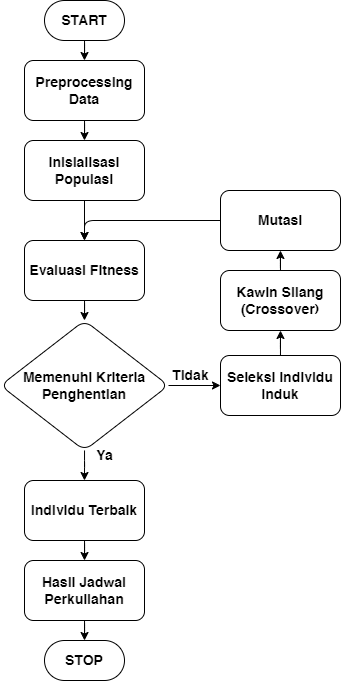
\includegraphics[scale=0.6]{gambar/metodologi.png}
  % Keterangan gambar yang diinputkan
  \caption{Metodologi Penelitian}
  % Label referensi dari gambar yang diinputkan
  \label{fig:metodologi}
\end{figure}

% Contoh penggunaan referensi dari gambar yang diinputkan
Penulis akan menggunakan beberapa metode untuk menyelesaikan penelitian tersebut. 
Metode yang digunakan dapat dilihat pada Gambar \ref*{fig:metodologi}

\subsection{Preprocessing Data dan Desain Kromosom}
  
  Pada penelitian ini, penulis akan menggunakan data dari Departemen Teknik Komputer ITS yang meliputi data mata kuliah, 
  jumlah ruangan, kapasitas masing-masing ruangan, jumlah dosen, dan jumlah mahasiswa. Data-data tersebut antara lain:
  \begin{longtable}{|c|l|}
    \caption{Dosen Departemen Teknik Komputer ITS}
    \label{tb:DosenTekkom} \\
    \hline
    \rowcolor[HTML]{C0C0C0} 
    No. & Dosen                                         \\ \hline
    1   & Dr. Eko Mulyanto Yuniarno, S.T.,M.T.          \\ 
    2   & Dr. Diah Puspito Wulandari, S.T.,M.Sc.        \\ 
    3   & Dr. I Ketut Eddy Purnama, S.T.,M.T.           \\ 
    4   & Ir. Hany Boedinugroho, M.T.                   \\ 
    5   & Prof. Dr. Ir. Yoyon Kusnendar Suprapto, M.Sc. \\ 
    6   & Prof. Dr. Ir. Mauridhi Hery Purnomo, M.Eng.   \\ 
    7   & Dr. Surya Sumpeno, S.T.,M.Sc.                 \\ 
    8   & Eko Pramunanto, S.T., M.T.                    \\ 
    9   & Arief Kurniawan, S.T., M.T.                   \\ 
    10  & Muhtadin, S.T., M.T.                          \\ 
    11  & Atar Fuady Babgei, S.T., M.Sc.                \\ 
    12  & Mochamad Hariadi, S.T.,M.Sc.,Ph.D             \\ 
    13  & Dr. Supeno Mardi Susiki Nugroho, S.T., M.T.   \\ 
    14  & Susi Juniastuti, S.T.,M.Eng.                  \\ 
    15  & Ahmad Zaini, S.T., M.Sc.                      \\ 
    16  & Reza Fuad Rachmadi, S.T.,M.T.,Ph.D            \\ 
    17  & Dion Hayu Fandiantoro, S.T., M.Eng.           \\ 
    \hline
  \end{longtable}

\begin{longtable}{|c|l|r|}
  \caption{Mata Kuliah Semester Genap 2022-2023 \linebreak Departemen Teknik Komputer ITS}
  \label{tb:matkul}\\
  \hline
  \rowcolor[HTML]{D0CECE} 
  No. & Mata Kuliah & Peserta \\ \hline
  1  & Aljabar Linear - A                            & 5  \\
  2  & Arsitektur dan Organisasi Sistem Komputer - A & 30 \\
  3  & Arsitektur dan Organisasi Sistem Komputer - B & 27 \\
  4  & Dasar Pemrograman - P                         & 14 \\
  5  & Deep Learning untuk Multimedia - A            & 19 \\
  6  & Desain dan Pemrograman Game - A               & 9  \\
  7  & Desain dan Pemrograman Game - P               & 8  \\
  8  & Desain Dan Rekayasa Sistem - A                & 49 \\
  9  & Desain Dan Rekayasa Sistem - B                & 40 \\
  10 & Jaringan Komputer - A                         & 41 \\
  11 & Jaringan Komputer - B                         & 40 \\
  12 & Matematika Diskrit - A                        & 32 \\
  13 & Matematika Diskrit - B                        & 59 \\
  14 & Metode Numerik - A                            & 40 \\
  15 & Metode Numerik - B                            & 40 \\
  16 & Metode Numerik - C                            & 59 \\
  17 & Pemrograman Lanjut - A                        & 39 \\
  18 & Pemrograman Lanjut - B                        & 39 \\
  19 & Pemrograman Sistem dan Jaringan - A           & 11 \\
  20 & Pengantar Robotika - A                        & 33 \\
  21 & Pengolahan Sinyal Digital - A                 & 26 \\
  22 & Pengolahan Sinyal Digital - B                 & 26 \\
  23 & Persamaan Differensial dan Deret - A          & 35 \\
  24 & Persepsi Robot - A                            & 13 \\
  25 & Probabilitas dan Statistik - A                & 28 \\
  26 & Rangkaian Digital - A                         & 24 \\
  27 & Rangkaian Listrik - A                         & 40 \\
  28 & Rangkaian Listrik - B                         & 35 \\
  29 & Sekuriti Sistem Komputer - A                  & 33 \\
  30 & Sistem Manajemen Basis Data - A               & 25 \\
  31 & Sistem Manajemen Basis Data - B               & 25 \\
  32 & Sistem Mikroprosesor dan Mikrokontroller - A  & 26 \\
  33 & Sistem Mikroprosesor dan Mikrokontroller - B  & 20 \\
  34 & Sistem Operasi - A                            & 25 \\
  35 & Sistem Operasi - B                            & 26 \\
  36 & Sistem Tertanam - A                           & 27 \\
  37 & Sistem Tertanam - B                           & 24 \\
  38 & Visi Komputer - A                             & 16 \\    
  \hline
\end{longtable}

\begin{longtable}{|c|l|r|}
  \caption{Ruang Kelas Departemen Teknik Komputer ITS}
  \label{tb:ruang}\\
  \hline
  \rowcolor[HTML]{D0CECE} 
  No. & Ruangan & Kapasitas \\ \hline
  1   & A108                                                 & 80                                                     \\ 
  2   & A234                                                 & 36                                                     \\ 
  3   & A235                                                 & 40                                                     \\ 
  4   & AJ401                                                & 25                                                     \\ 
  5   & AJ402                                                & 25                                                     \\ 
  6   & B211                                                 & 25                                                     \\ 
  7   & PASCA 2                                              & 40                                                     \\ 
  \hline
\end{longtable}

\begin{longtable}[c]{|c|c|}
  \caption{Waktu Perkuliahan Semester Genap 2022-2023 Departemen Teknik Komputer ITS}
  \label{waktu}\\
  \hline
  \rowcolor[HTML]{D0CECE} 
  Hari                    & Waktu       \\ \hline
  \multirow{3}{*}{Senin}  & 07.30-10.00 \\ \cline{2-2} 
                          & 10.00-12.30 \\ \cline{2-2} 
                          & 13.30-16.00 \\ \hline
  \multirow{3}{*}{Selasa} & 07.30-10.00 \\ \cline{2-2} 
                          & 10.00-12.30 \\ \cline{2-2} 
                          & 13.30-16.00 \\ \hline
  \multirow{3}{*}{Rabu}   & 07.30-10.00 \\ \cline{2-2} 
                          & 10.00-12.30 \\ \cline{2-2} 
                          & 13.30-16.00 \\ \hline
  \multirow{3}{*}{Kamis}  & 07.30-10.00 \\ \cline{2-2} 
                          & 10.00-12.30 \\ \cline{2-2} 
                          & 13.30-16.00 \\ \hline
  \multirow{3}{*}{Jumat}  & 07.30-10.00 \\ \cline{2-2} 
                          & 10.00-12.30 \\ \cline{2-2} 
                          & 13.30-16.00 \\ \hline
  \end{longtable}
  Data-data tersebut kemudian diolah sedemikian rupa sesuai dengan desain kromosom \linebreak sehingga dapat digunakan dalam proses algoritma genetika. Desain kromosom yang digunakan adalah sebagai berikut:
\begin{figure} [ht] \centering
    % Nama dari file gambar yang diinputkan
    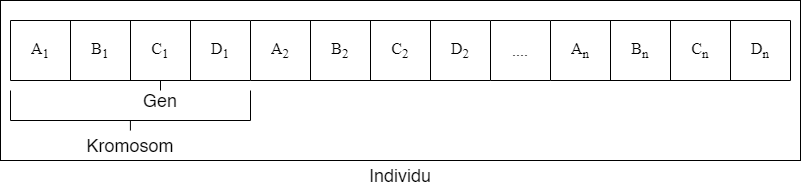
\includegraphics[scale=0.5]{gambar/kromosom.png}
    % Keterangan gambar yang diinputkan
    \caption{Desain Kromosom}
    % Label referensi dari gambar yang diinputkan
    \label{fig:kromosom}
\end{figure}\\
  Keterangan:\\
  A = Dosen\\
  B = Mata Kuliah\\
  C = Ruangan\\
  D = Waktu\\
  n = Kromosom ke-n

Sedangkan untuk proses pengkodean gen digunakan metode permutasi dengan \linebreak membangkitkan angka secara acak yang mewakili urutan masing-masing data yang \linebreak direpresentasikan oleh masing-masing gen.

\subsection{Inisialisasi Populasi}
Hal pertama yang dilakukan dalam program penjadwalan ini adalah pembangkitan \linebreak individu-individu induk sesuai dengan desain kromosom yang telah dibuat sebelumnya. Individu ini berbentuk \emph{nested list} yang berisi list gen didalam list kromosom dalam satu kesatuan individu.  
\begin{lstlisting}[
  language=Python,
  caption={Fungsi pembangkitan individu},
  label={lst:Populasi}
  ]
  def create_individu():
  individu = [[random.randint(1, len(Dosen.dosen)), 
              i+1,
               random.randint(1, len(Ruang.ruang)),
               random.randint(1, len(Waktu.waktu))
               ] 
              for i in range (len(Matkul.matkul))]
  return individu
\end{lstlisting}
Panjang kromosom untuk masing-masing individu sesuai dengan banyaknya mata kuliah yang akan dilaksanakan dalam satu semester perkuliahan.
\subsection{Evaluasi Fitness}
  
  Individu-individu yang ada dievaluasi dengan fungsi fitness untuk menentukan kecocokan dengan batasan yang telah ditentukan sebelumnya. 
  Fungsi fitness yang digunakan adalah sebagai berikut:
  
  \begin{equation}
    \label{eq:fitness2}
    \mathbf{Fitness} = \frac{1}{(1 + (F1 + F2 + \cdot \cdot \cdot +  Fn))}\; 
  \end{equation}\\
  Keterangan:\\
  Fn = Banyaknya Konflik\\
  n  = Batasan ke-n\\

  Fungsi \ref{eq:fitness2} akan menghitung banyaknya konflik yang ada pada satu individu. Konflik ini berupa pelanggaran pada batasan yang telah ditentukan sebelumnya.
  Batasan-batasan tersebut antara lain:
  \begin{enumerate}
    \item Satu mata kuliah hanya bisa diselenggarakan satu kali dalam satu minggu
    \item Satu ruangan hanya bisa dipakai satu kali dalam satu waktu
    \item Satu dosen hanya bisa mengajar satu kali dalam satu waktu
    \item Jumlah peserta perkuliahan tidak boleh melebihi kapasitas ruangan
  \end{enumerate} 
 Pada proses penghitungan konflik, nilai 1 ditambahkan untuk menghindari hasil tak hingga ketika tidak ada pelanggaran sama sekali. 
 Semakin besar nilai fitness yang dihasilkan, maka semakin baik individu tersebut dan semakin cocok dengan hasil penjadwalan yang diharapkan. 
\subsection{Pemilihan Individu Induk}
  
  Individu-individu yang telah melalui proses evaluasi dipilih untuk dijadikan sebagai \linebreak induk untuk proses crossover.
  Metode yang digunakan dalam proses seleksi ini adalah metode \linebreak rangking, dimana individu dengan fitness terbaik digunakan sebagai individu induk untuk proses selanjutnya. 
  Proses pemilihan individu induk dilakukan dengan program dibawah ini:
  \begin{lstlisting}[
    language=Python,
    caption={Fungsi pemilihan individu induk},
    label={lst:selection}
    ]
    def selection(a,b,c,d,e,f):
      pop = [a,b,c,d,e,f]

      sorted_pop = sorted(pop, key=lambda x: fitness(x), reverse=True)
      
      x1 = sorted_pop[0]
      x2 = sorted_pop[1]
      fit = fitness(x1)

    return x1,x2,fitness(x1)
  \end{lstlisting}
  Fungsi ini akan mengembalikan 2 individu terbaik dari total 6 individu yang dimasukkan, sekaligus mengembalikan nilai fitness dari individu terbaik. 
  Individu yang dikembalikan ini digunakan untuk proses \emph{loop} berikutnya dan nilai fitness ini digunakan untuk kebutuhan penghentian proses penjadwalan otomatis ini.
\subsection{\emph{Crossover}}
  
Crossover atau pindah silang adalah salah satu komponen algoritma genetika yang \linebreak berfungsi untuk mendapatkan solusi dengan melakukan pindah silang kromosom-kromosom dari dua buah individu yang biasa disebut \emph{parent}. 
Proses ini akan menghasilkan 2 individu baru yang disebut dengan \emph{child}. Proses \emph{crossover} dilakukan dengan skema sesuai gambar dibawah ini:
% \begin{lstlisting}[
%   language=Python,
%   caption={Fungsi crossover},
%   label={lst:crossover},
%   ]
%   def crossover(a,b):
%     a = list(a)
%     b = list(b)
%     n = random.randint(1, (len(a)-1))
%     m = random.randint(n, (len(a)-1))

%     for i in range (n, m):
%       a[i],b[i] = b[i],a[i]

%   return a,b
% \end{lstlisting}
\begin{figure} [ht] \centering
  % Nama dari file gambar yang diinputkan
  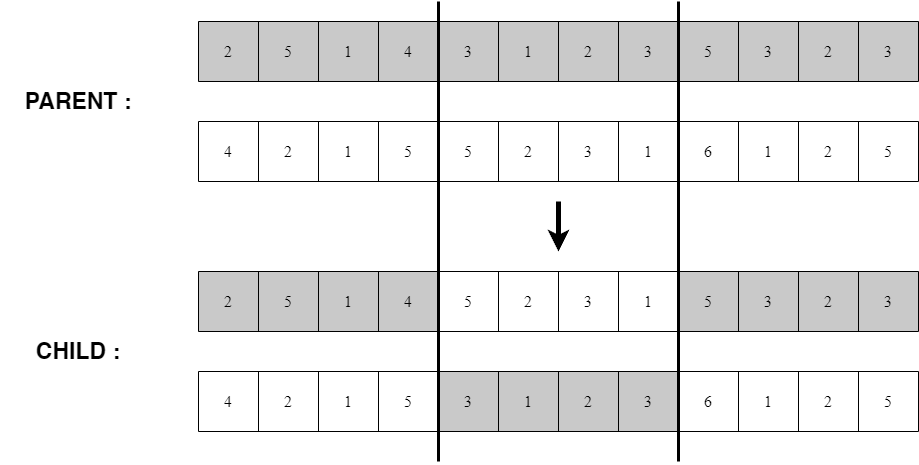
\includegraphics[scale=0.4]{gambar/cross.png}
  % Keterangan gambar yang diinputkan
  \caption{Two Points Crossover}
  % Label referensi dari gambar yang diinputkan
  \label{fig:cross}
\end{figure}

Pada proses crossover ini digunakan 2 titik crossover berupa angka yang dibangkitkan secara random.
Kromosom yang berada diantara 2 titik tersebut, dipindahkan antara satu induk dengan induk yang lain sehingga menghasilkan 2 individu baru.
\emph{Child} atau individu baru yang dihasilkan dari proses ini akan diteruskan ke proses mutasi.

\subsection{Mutasi}
  
  Mutasi merupakan proses dalam algoritma genetika yang bertujuan untuk mengubah isi gen dalam sebuah kromosom secara acak. 
  Tidak semua individu baru hasil crossover \linebreak mengalami proses mutasi. 
  Individu-individu baru akan mengalami mutasi atau tidak, ditentukan oleh probabilitas mutasi dari proses algoritma genetika yang telah ditentukan sebelumnya. 
  Proses mutasi dilakukan dengan program berikut ini:
  \begin{lstlisting}[
    language=Python,
    caption={Fungsi mutasi},
    label={lst:mutasi},
    ]
    def gA(a,b,rate):
      generation = 0
      score = 0.00
      while True:
        if generation == 200000 or score == 1.00:
          
          break
        else:
          print("Generation: ", generation)
          c,d = crossover(a,b)
          e,f = mutate(c,d,rate)
          a,b,fit = selection(a,b,c,d,e,f)
          
          print("Fitness a:", fitness(a))
          print("Fitness b:", fitness(b))
          print("\n")
          score = fit
          generation = generation+1

      return a    
  \end{lstlisting}
  Untuk menentukan proses mutasi berjalan atau tidak, dilakukan dengan cara membangkitkan angka secara acak antara 0 hingga 1. 
  Jika angka yang dibangkitkan memiliki nilai dibawah probabilitas mutasi, maka proses mutasi akan terjadi.
  \begin{figure} [ht] \centering
    % Nama dari file gambar yang diinputkan
    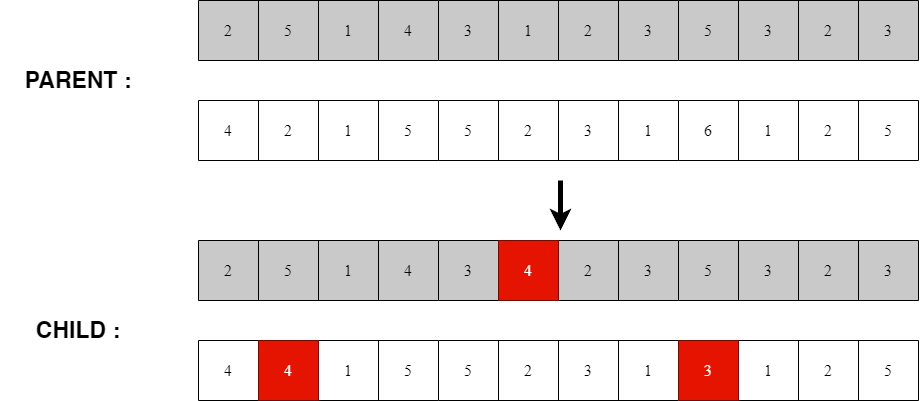
\includegraphics[scale=0.4]{gambar/mutation.png}
    % Keterangan gambar yang diinputkan
    \caption{Proses Mutasi}
    % Label referensi dari gambar yang diinputkan
    \label{fig:mutate}
  \end{figure}

  Proses mutasi akan membangkitkan ulang nilai gen-gen pada sebuah cromosom secara acak (Gambar \ref{fig:mutate}). Penentuan posisi kromosom yang dimutasi juga dilakukan secara acak dengan membangkitkan angka dalam jangkauan tertentu. 
  Proses mutasi ini menghasilkan 2 individu baru.
  \subsection{Kriteria Penghentian}
  
  Proses algoritma genetika hanya akan berhenti jika telah memenuhi kriteria penghentian yang telah ditentukan sebelumnya. 
  Kriteria penghentian ini dapat berupa nilai fitness tertentu, atau jumlah iterasi tertentu. 
  Jika nilai fitness telah terpenuhi atau jumlah iterasi telah terlewati, maka proses algoritma genetika akan berhenti.

\section{Bahan dan Peralatan yang Digunakan}
Dalam penelitian ini akan digunakan beberapa perangkat yang dibutuhkan untuk menunjang berjalannya penelitian dengan baik.
Berikut merupakan hardware dan software yang digunakan dalam melakukan proses pembuatan program sekaligus pengujian program yang digunakan pada penelitian ini.
\subsection{\emph{Hardware}}
Perangkat komputer yang digunakan untuk pengerjaan tugas akhir ini antara lain \emph{Asus TUF FX 505 DT} dengan spesifikasi \emph{AMD Ryzen 5 R5-3550H Processor, GeForce GTX 1650 Graphics, 16GB DDR4, 1TB HDD, 512GB SSD,} dan \emph{Windows 11 64-bit}.
\subsection{\emph{Software}}
\emph{Software} yang digunakan dalam penelitian ini adalah \emph{Jupyter Notebook} dan \emph{Google Colab}.

\section{Urutan Pelaksanaan Penelitian}
% Ubah tabel berikut sesuai dengan isi dari rencana kerja
\newcommand{\w}{}
\newcommand{\G}{\cellcolor{gray}}
\begin{table}[h!]
  \caption{Tabel timeline}
  \label{tb:timeline}
  \begin{tabular}{|p{3.5cm}|c|c|c|c|c|c|c|c|c|c|c|c|c|c|c|c|}

    \hline
    \multirow{2}{*}{Kegiatan} & \multicolumn{16}{|c|}{Minggu} \\
    \cline{2-17} &
    1 & 2 & 3 & 4 & 5 & 6 & 7 & 8 & 9 & 10 & 11 & 12 & 13 & 14 & 15 & 16 \\
    \hline

    % Gunakan \G untuk mengisi sel dan \w untuk mengosongkan sel
    Studi Literatur &
    \G & \G & \w & \w & \w & \w & \w & \w & \w & \w & \w & \w & \w & \w & \w & \w \\
    \hline

    Pengumpulan Data &
    \w & \G & \G & \w & \w & \w & \w & \w & \w & \w & \w & \w & \w & \w & \w & \w \\
    \hline

    Preprocessing Data &
    \w & \w & \G & \G & \G & \w & \w & \w & \w & \w & \w & \w & \w & \w & \w & \w \\
    \hline

    Pembuatan Program &
    \w & \w & \w & \w & \G & \G & \G & \G & \G & \G & \G & \G & \w & \w & \w & \w \\
    \hline

    Pengujian Program &
    \w & \w & \w & \w & \w & \w & \w & \w & \w & \w & \w & \G & \G & \G & \w & \w \\
    \hline

    Penyusunan \linebreak Laporan &
    \G & \G & \G & \G & \G & \G & \G & \G & \G & \G & \G & \G & \G & \G & \G & \G \\
    \hline

  \end{tabular}
\end{table}
% \section{Bahan dan Alat yang Digunakan}
%   \label{sec:bahan dan alat}

% Alat diimplementasikan dengan \lipsum[1]

% Contoh pembuatan potongan kode
% \begin{lstlisting}[
%   language=C++,
%   caption={Program halo dunia.},
%   label={lst:halodunia}
% ]
% #include <iostream>

% int main() {
%     std::cout << "Halo Dunia!";
%     return 0;
% }
% \end{lstlisting}

% \lipsum[2-3]

% % Contoh input potongan kode dari file
% \lstinputlisting[
%   language=Python,
%   caption={Program perhitungan bilangan prima.},
%   label={lst:bilanganprima}
% ]{program/bilangan-prima.py}

% \lipsum[4]

\cleardoublepage

% Bab 4 pengujian dan analisis
\chapter{HASIL DAN PEMBAHASAN}
\label{chap:hasilpembahasan}

% Ubah bagian-bagian berikut dengan isi dari pengujian dan analisis

% Pada penelitian ini dipaparkan \lipsum[1][1-5]

\section{Hasil Penelitian}
\label{sec:hasil penelitian}
Sistem yang sudah dibuat mampu menghasilkan individu yang memenuhi batasan-batasan yang telah ditentukan sebelumnya dan individu terbaik dapat menghasilkan nilai fitness 1.00. Nilai fitness 1.00 berarti tidak ada batasan yang dilanggar. Contoh hasil keluaran program penjadwalan otomatis ini adalah sebagai berikut:
 
% \begin{lstlisting}[language=Python,caption={Output penjadwalan otomatis}]
%   Generation:  105831
%   3
%   Mutate
%   Fitness a: 1.0
%   Fitness b: 1.0
%   Chromosome terbaik: 
%   [[10, 2, 3, 1], [9, 26, 4, 1], [17, 9, 5, 1], [11, 5, 2, 3], [7, 18, 3, 3], [6, 12, 5, 3], [10, 25, 3, 4], [15, 32, 4, 4], [12, 28, 5, 4], [2, 35, 2, 5], [3, 16, 4, 5], [9, 10, 6, 5], [9, 6, 7, 6], [14, 1, 1, 6], [17, 14, 3, 6], [2, 4, 2, 6], [10, 27, 4, 6], [13, 37, 1, 7], [4, 33, 7, 7], [5, 22, 5, 7], [1, 11, 4, 7], [11, 21, 2, 8], [7, 13, 4, 8], [3, 30, 7, 8], [2, 24, 5, 9], [9, 29, 4, 10], [17, 20, 4, 11], [5, 7, 6, 11], [16, 17, 3, 12], [11, 38, 6, 12], [4, 3, 5, 12], [2, 8, 4, 12], [6, 15, 4, 13], [11, 34, 2, 14], [3, 36, 4, 14], [14, 31, 7, 14], [13, 19, 6, 14], [2, 23, 3, 14]]
% \end{lstlisting}
\begin{longtable}[c]{|c|c|c|>{\centering\arraybackslash}m{3cm}|>{\centering\arraybackslash}m{3cm}|}
  \caption{Hasil Penjadwalan Otomatis}
  \label{tab:jadwal}\\
  \hline
  Hari   & Waktu       & Ruang                  & Matkul                                                              & Dosen                                         \\ \hline
  \rowcolor[HTML]{DAE8FC} 
  Senin  & 07.30-10.00 & A235, Kapasitas: 40    & Aljabar Linear A, \linebreak Peserta: 5                             & Muhtadin, S.T., M.T.                          \\ \hline
  \rowcolor[HTML]{DAE8FC} 
  Senin  & 07.30-10.00 & A108, Kapasitas: 80    & Rangkaian Digital A, \linebreak Peserta: 24                         & Arief Kurniawan, S.T., M.T.                   \\ \hline
  \rowcolor[HTML]{DAE8FC} 
  Senin  & 07.30-10.00 & Pasca 2, Kapasitas: 40 & Desain Dan Rekayasa Sistem B, \linebreak Peserta: 40                & Dion Hayu Fandiantoro, S.T., M.Eng.           \\ \hline
  \rowcolor[HTML]{DAE8FC} 
  Senin  & 13.30-16.00 & A234, Kapasitas: 36    & Deep Learning untuk Multimedia A, \linebreak Peserta: 30            & Atar Fuady Babgei, S.T., M.Sc.                \\ \hline
  \rowcolor[HTML]{DAE8FC} 
  Senin  & 13.30-16.00 & A235, Kapasitas: 40    & Pemrograman Lanjut B, \linebreak Peserta: 39                        & Dr. Surya Sumpeno, S.T.,M.Sc.                 \\ \hline
  \rowcolor[HTML]{DAE8FC} 
  Senin  & 13.30-16.00 & Pasca 2, Kapasitas: 40 & Matematika Diskrit A, \linebreak Peserta: 32                        & Prof. Dr. Ir. Mauridhi Hery Purnomo, M.Eng.   \\ \hline
  Selasa & 07.30-10.00 & A235, Kapasitas: 40    & Probabilitas dan Statistik A, \linebreak Peserta: 28                & Muhtadin, S.T., M.T.                          \\ \hline
  Selasa & 07.30-10.00 & A108, Kapasitas: 80    & Sistem Mikroprosesor dan Mikrokontroller A, \linebreak Peserta: 26  & Ahmad Zaini, S.T., M.Sc.                      \\ \hline
  Selasa & 07.30-10.00 & Pasca 2, Kapasitas: 40 & Rangkaian Listrik B, \linebreak Peserta: 35                         & Mochamad Hariadi, S.T.,M.Sc.,Ph.D             \\ \hline
  Selasa & 10.00-12.30 & A234, Kapasitas: 36    & Sistem Operasi B, \linebreak Peserta: 26                            & Dr. Diah Puspito Wulandari, S.T.,M.Sc.        \\ \hline
  Selasa & 10.00-12.30 & A108, Kapasitas: 80    & Metode Numerik C, \linebreak Peserta: 59                            & Dr. I Ketut Eddy Purnama, S.T.,M.T.           \\ \hline
  Selasa & 10.00-12.30 & AJ401, Kapasitas: 25   & Jaringan Komputer A, \linebreak Peserta: 41                         & Arief Kurniawan, S.T., M.T.                   \\ \hline
  Selasa & 13.30-16.00 & AJ402, Kapasitas: 25   & Desain Pemrograman Game A, \linebreak Peserta: 9                    & Arief Kurniawan, S.T., M.T.                   \\ \hline
  Selasa & 13.30-16.00 & B211, Kapasitas: 25    & Dasar Pemrograman P, \linebreak Peserta: 14                         & Susi Juniastuti, S.T.,M.Eng.                  \\ \hline
  Selasa & 13.30-16.00 & A235, Kapasitas: 40    & Metode Numerik A, \linebreak Peserta: 40                            & Dion Hayu Fandiantoro, S.T., M.Eng.           \\ \hline
  Selasa & 13.30-16.00 & A234, Kapasitas: 36    & Arsitektur dan Organisasi Sistem Komputer B, \linebreak Peserta: 27 & Dr. Diah Puspito Wulandari, S.T.,M.Sc.        \\ \hline
  Selasa & 13.30-16.00 & A108, Kapasitas: 80    & Rangkaian Listrik A, \linebreak Peserta: 40                         & Muhtadin, S.T., M.T.                          \\ \hline
  \rowcolor[HTML]{DAE8FC} 
  Rabu   & 07.30-10.00 & B211, Kapasitas: 25    & Sistem Tertanam B, \linebreak Peserta: 24                           & Dr. Supeno Mardi Susiki Nugroho, S.T., M.T.   \\ \hline
  \rowcolor[HTML]{DAE8FC} 
  Rabu   & 07.30-10.00 & AJ402, Kapasitas: 25   & Sistem Mikroprosesor dan Mikrokontroller B, \linebreak Peserta: 20  & Ir. Hany Boedinugroho, M.T.                   \\ \hline
  \rowcolor[HTML]{DAE8FC} 
  Rabu   & 07.30-10.00 & Pasca 2, Kapasitas: 40 & Pengolahan Sinyal Digital B, \linebreak Peserta: 26                 & Prof. Dr. Ir. Yoyon Kusnendar Suprapto, M.Sc. \\ \hline
  \rowcolor[HTML]{DAE8FC} 
  Rabu   & 07.30-10.00 & A108, Kapasitas: 80    & Jaringan Komputer B, \linebreak Peserta: 40                         & Dr. Eko Mulyanto Yuniarno, S.T.,M.T.          \\ \hline
  \rowcolor[HTML]{DAE8FC} 
  Rabu   & 10.00-12.30 & A234, Kapasitas: 36    & Pengolahan Sinyal Digital A, \linebreak Peserta: 26                 & Atar Fuady Babgei, S.T., M.Sc.                \\ \hline
  \rowcolor[HTML]{DAE8FC} 
  Rabu   & 10.00-12.30 & A108, Kapasitas: 80    & Matematika Diskrit B, \linebreak Peserta: 59                        & Dr. Surya Sumpeno, S.T.,M.Sc.                 \\ \hline
  \rowcolor[HTML]{DAE8FC} 
  Rabu   & 10.00-12.30 & AJ402, Kapasitas: 25   & Sistem Manajemen Basis Data A, \linebreak Peserta: 25               & Dr. I Ketut Eddy Purnama, S.T.,M.T.           \\ \hline
  \rowcolor[HTML]{DAE8FC} 
  Rabu   & 13.30-16.00 & Pasca 2, Kapasitas: 40 & Persepsi Robot A, \linebreak Peserta: 13                            & Dr. Diah Puspito Wulandari, S.T.,M.Sc.        \\ \hline
  Kamis  & 07.30-10.00 & A108, Kapasitas: 80    & Sekuriti Sistem Komputer A, \linebreak Peserta: 33                  & Arief Kurniawan, S.T., M.T.                   \\ \hline
  Kamis  & 10.00-12.30 & A108, Kapasitas: 80    & Pengantar Robotika A, \linebreak Peserta: 33                        & Dion Hayu Fandiantoro, S.T., M.Eng.           \\ \hline
  Kamis  & 10.00-12.30 & AJ401, Kapasitas: 25   & Desain Pemrograman Game P, \linebreak Peserta: 8                    & Prof. Dr. Ir. Yoyon Kusnendar Suprapto, M.Sc. \\ \hline
  Kamis  & 13.30-16.00 & A235, Kapasitas: 40    & Pemrograman Lanjut A, \linebreak Peserta: 39                        & Reza Fuad Rachmadi, S.T.,M.T.,Ph.D            \\ \hline
  Kamis  & 13.30-16.00 & AJ401, Kapasitas: 25   & Visi Komputer A, \linebreak Peserta: 16                             & Atar Fuady Babgei, S.T., M.Sc.                \\ \hline
  Kamis  & 13.30-16.00 & Pasca 2, Kapasitas: 40 & Arsitektur dan Organisasi Sistem Komputer A, \linebreak Peserta: 30 & Ir. Hany Boedinugroho, M.T.                   \\ \hline
  Kamis  & 13.30-16.00 & A108, Kapasitas: 80    & Desain Dan Rekayasa Sistem A, \linebreak Peserta: 49                & Dr. Diah Puspito Wulandari, S.T.,M.Sc.        \\ \hline
  \rowcolor[HTML]{DAE8FC} 
  Jumat  & 07.30-10.00 & A108, Kapasitas: 80    & Metode Numerik B, \linebreak Peserta: 40                            & Prof. Dr. Ir. Mauridhi Hery Purnomo, M.Eng.   \\ \hline
  \rowcolor[HTML]{DAE8FC} 
  Jumat  & 13.30-16.00 & A234, Kapasitas: 36    & Sistem Operasi A, \linebreak Peserta: 25                            & Atar Fuady Babgei, S.T., M.Sc.                \\ \hline
  \rowcolor[HTML]{DAE8FC} 
  Jumat  & 13.30-16.00 & A108, Kapasitas: 80    & Sistem Tertanam A, \linebreak Peserta: 27                           & Dr. I Ketut Eddy Purnama, S.T.,M.T.           \\ \hline
  \rowcolor[HTML]{DAE8FC} 
  Jumat  & 13.30-16.00 & AJ402, Kapasitas: 25   & Sistem Manajemen Basis Data B, \linebreak Peserta: 25               & Susi Juniastuti, S.T.,M.Eng.                  \\ \hline
  \rowcolor[HTML]{DAE8FC} 
  Jumat  & 13.30-16.00 & AJ401, Kapasitas: 25   & Pemrograman Sistem dan Jaringan A, \linebreak Peserta: 11           & Dr. Supeno Mardi Susiki Nugroho, S.T., M.T.   \\ \hline
  \rowcolor[HTML]{DAE8FC} 
  Jumat  & 13.30-16.00 & A235, Kapasitas: 40    & Persamaan Differensial dan Deret A, \linebreak Peserta: 35          & Dr. Diah Puspito Wulandari, S.T.,M.Sc.        \\ \hline
\end{longtable}
Hasil keluaran program diatas merupakan hasil keluaran dari percobaan penjadwalan otomatis yang memperhatikan kapasitas ruangan dan jumlah peserta tiap mata kuliah dan menggunakan probabilitasan percobaan yang memperhatikan probabilitasis mutasi sebesar 0.05. Percobaan ini memakan waktu 14 menit 52 detik.

Terdapat dua percobaan yang dilakukan dalam sistem penjadwalan otomatis ini. Percobaan pertama yaitu tanpa memperhatikan kapasitas kelas dan jumlah perserta tiap mata kuliah, dan percobaan kedua dengan memperhatikan kapasitas ruang kelas dan jumlah perserta tiap mata kuliah.
Masing-masing percobaan dilakukan dengan memvariasikan probabilitas mutasi yaitu dengan nilai 0.04, 0.05, dan 0.06.
Masing-masing percobaan dilakukan dengan 5 kali \emph{loop} pada konfigurasi yang sama. 
Hasil percobaan yang telah dilakukan dapat dilihat pada tabel dibawah ini:
\begin{longtable}{|c|c|}
  \caption{Percobaan tanpa memperhatikan kapasitas \linebreak ruang dan jumlah peserta mata kuliah}
  \label{tab:tanpaKapasitas}\\
  \hline
  \rowcolor[HTML]{C0C0C0} 
{\color[HTML]{000000} \textbf{Probabilitas Mutasi}} & {\color[HTML]{000000} \textbf{Rata-Rata Waktu}} \\ \hline
0.04                                                & 6m 46s                                           \\ \hline
0.05                                                & 5m 38s                                           \\ \hline
0.06                                                & 4m 54s                                           \\ \hline
\end{longtable}

\begin{longtable}{|c|c|}
  \caption{Percobaan dengan memperhatikan kapasitas \linebreak ruang dan jumlah peserta mata kuliah}
  \label{tab:denganKapasitas}\\
  \hline
  \rowcolor[HTML]{C0C0C0} 
{\color[HTML]{000000} \textbf{Probabilitas Mutasi}} & {\color[HTML]{000000} \textbf{Rata-Rata Waktu}} \\ \hline
0.04                                                & 39m 43s                                         \\ \hline
0.05                                                & 14m 53s                                         \\ \hline
0.06                                                & 23m 18s                                         \\ \hline
\end{longtable}


% Pengujian dilakukan dengan memvariasikan nilai probabilitas mutasi yang kemudian diperoleh rataan waktu untuk menyelesaikan proses penjadwalan. 
% Tabel rata-rata waktu proses penjadwalan adalah sebagai berikut.
% \begin{longtable}{|c|c|}
%   \caption{Hasil Percobaan Variasi Probabilitas Mutasi}
%   \label{tab:variasiMutasi}\\
%   \hline
%   \rowcolor[HTML]{C0C0C0} 
%   {\color[HTML]{000000} \textbf{Probabilitas Mutasi}} & {\color[HTML]{000000} \textbf{Rata-Rata Waktu}} \\ \hline
%   0.04                                                & 39m 43s                                         \\ \hline
%   0.05                                                & 14m 53s                                         \\ \hline
%   0.06                                                & 23m 18s                                         \\ \hline
% \end{longtable}
\section{Pembahasan}
\label{sec:Pembahasan}

Dari pengujian yang telah dilakukan dapat diketahui bahwa semakin banyak batasan-batasan yang diberikan dalam proses algoritma genetika, maka kompleksitas dari proses perhitungan evaluasi fitness juga akan semakin rumit. 
Kerumitan proses perhitungan ini tentu akan menambah durasi dari proses algoritma genetika itu sendiri. Hal ini dapat dilihat dari perbedaan waktu antara Tabel \ref{tab:tanpaKapasitas} dengan Tabel \ref{tab:denganKapasitas}.

Selain kompleksitas perhitungan evaluasi fitness dari satu individu, penentuan probabilitas mutasi juga sangat berpengaruh terhadap durasi proses algoritma genetika. Probabilitas \linebreak mutasi dalam sebuah proses algoritma genetika tidak boleh terlalu besar, karena mengakibatkan hilangnya kemiripan antara individu baru dengan individu induknya. 
Sedangkan jika probabilitas mutasi bernilai terlalu kecil, maka durasi untuk memperoleh solusi berupa individu terbaik, akan memakan waktu yang sangat lama dan membuat proses algorima genetika dari penjadwalan otomatis ini menjadi tidak optimal. 

Data yang diperoleh pada Tabel \ref{tab:tanpaKapasitas} menunjukkan bahwa probabilitas mutasi 0.06 memiliki rata-rata durasi yang paling singkat yaitu dengan waktu 4 menit 54 detik. Sedangkan data pada Tabel \ref{tab:denganKapasitas} menunjukkan bahwa probabilitas mutasi 0.05 memiliki rata-rata durasi yang paling singkat yakni dengan waktu 14 menit 53 detik. 
% Contoh pembuatan tabel
% \begin{longtable}{|c|c|c|}
%   \caption{Hasil Pengukuran Energi dan Kecepatan}
%   \label{tb:EnergiKecepatan}                                   \\
%   \hline
%   \rowcolor[HTML]{C0C0C0}
%   \textbf{Energi} & \textbf{Jarak Tempuh} & \textbf{Kecepatan} \\
%   \hline
%   10 J            & 1000 M                & 200 M/s            \\
%   20 J            & 2000 M                & 400 M/s            \\
%   30 J            & 4000 M                & 800 M/s            \\
%   40 J            & 8000 M                & 1600 M/s           \\
%   \hline
% \end{longtable}

% \lipsum[2-4]

\cleardoublepage

% Bab 5 penutup
\chapter{PENUTUP}
\label{chap:penutup}

% Ubah bagian-bagian berikut dengan isi dari penutup

\section{Kesimpulan}
\label{sec:kesimpulan}

% Berdasarkan hasil pengujian yang \lipsum[1][1-3] sebagai berikut:

% \begin{enumerate}[nolistsep]

%   \item Pembuatan \lipsum[2][1-3]

%   \item \lipsum[2][4-6]

%   \item \lipsum[2][7-10]

% \end{enumerate}

\section{Saran}
\label{chap:saran}

% Untuk pengembangan lebih lanjut pada \lipsum[1][1-3] antara lain:

% \begin{enumerate}[nolistsep]

%   \item Memperbaiki \lipsum[2][1-3]

%   \item \lipsum[2][4-6]

%   \item \lipsum[2][7-10]

% \end{enumerate}

\cleardoublepage

\chapter*{DAFTAR PUSTAKA}
\addcontentsline{toc}{chapter}{DAFTAR PUSTAKA}
\renewcommand\refname{}
\vspace{2ex}
\renewcommand{\bibname}{}
\begingroup
\def\chapter*#1{}
\printbibliography
\endgroup
\cleardoublepage

% \begin{center}
    \Large
    \textbf{LAMPIRAN}
  \end{center}
  % Please add the following required packages to your document preamble:
% \usepackage{multirow}
\begin{table}[]
  \centering
  \caption{}
  \label{tab:my-table}
  \begin{tabular}{|c|c|ccccccc|}
  \hline
  \multirow{2}{*}{Hari}   & \multirow{2}{*}{Waktu}       & \multicolumn{7}{c|}{Ruang}                                                                                                                                                                                                                                                                                                                                                                                                                                               \\ \cline{3-9} 
                          &                              & \multicolumn{1}{c|}{A108}                                         & \multicolumn{1}{c|}{A234}                                          & \multicolumn{1}{c|}{A235}                                     & \multicolumn{1}{c|}{AJ401}                                           & \multicolumn{1}{c|}{AJ402}                                        & \multicolumn{1}{c|}{B211}                                          & PASCA 2                                         \\ \hline
  \multirow{6}{*}{Senin}  & \multirow{2}{*}{07.00-10.00} & \multicolumn{1}{c|}{Rangkaian Digital A}                          & \multicolumn{1}{c|}{}                                              & \multicolumn{1}{c|}{Aljabar Linear A}                         & \multicolumn{1}{c|}{}                                                & \multicolumn{1}{c|}{}                                             & \multicolumn{1}{c|}{}                                              & Desain Dan Rekayasa   Sistem B                  \\ \cline{3-9} 
                          &                              & \multicolumn{1}{c|}{Arief Kurniawan, S.T., M.T.}                  & \multicolumn{1}{c|}{}                                              & \multicolumn{1}{c|}{Muhtadin, S.T., M.T.}                     & \multicolumn{1}{c|}{}                                                & \multicolumn{1}{c|}{}                                             & \multicolumn{1}{c|}{}                                              & Dion Hayu   Fandiantoro, S.T., M.Eng.           \\ \cline{2-9} 
                          & \multirow{2}{*}{10.00-12.30} & \multicolumn{1}{c|}{}                                             & \multicolumn{1}{c|}{}                                              & \multicolumn{1}{c|}{}                                         & \multicolumn{1}{c|}{}                                                & \multicolumn{1}{c|}{}                                             & \multicolumn{1}{c|}{}                                              &                                                 \\ \cline{3-9} 
                          &                              & \multicolumn{1}{c|}{}                                             & \multicolumn{1}{c|}{}                                              & \multicolumn{1}{c|}{}                                         & \multicolumn{1}{c|}{}                                                & \multicolumn{1}{c|}{}                                             & \multicolumn{1}{c|}{}                                              &                                                 \\ \cline{2-9} 
                          & \multirow{2}{*}{13.30-16.00} & \multicolumn{1}{c|}{}                                             & \multicolumn{1}{c|}{Deep Learning untuk   Multimedia A}            & \multicolumn{1}{c|}{Pemrograman Lanjut B}                     & \multicolumn{1}{c|}{}                                                & \multicolumn{1}{c|}{}                                             & \multicolumn{1}{c|}{}                                              & Matematika Diskrit A                            \\ \cline{3-9} 
                          &                              & \multicolumn{1}{c|}{}                                             & \multicolumn{1}{c|}{Atar Fuady Babgei,   S.T., M.Sc.}              & \multicolumn{1}{c|}{Dr. Surya Sumpeno,   S.T.,M.Sc.}          & \multicolumn{1}{c|}{}                                                & \multicolumn{1}{c|}{}                                             & \multicolumn{1}{c|}{}                                              & Prof. Dr. Ir.   Mauridhi Hery Purnomo, M.Eng.   \\ \hline
  \multirow{6}{*}{Selasa} & \multirow{2}{*}{07.00-10.00} & \multicolumn{1}{c|}{Sistem Mikroprosesor   dan Mikrokontroller A} & \multicolumn{1}{c|}{}                                              & \multicolumn{1}{c|}{Probabilitas dan   Statistik A}           & \multicolumn{1}{c|}{}                                                & \multicolumn{1}{c|}{}                                             & \multicolumn{1}{c|}{}                                              & Rangkaian Listrik B                             \\ \cline{3-9} 
                          &                              & \multicolumn{1}{c|}{Ahmad Zaini, S.T., M.Sc.}                     & \multicolumn{1}{c|}{}                                              & \multicolumn{1}{c|}{Muhtadin, S.T., M.T.}                     & \multicolumn{1}{c|}{}                                                & \multicolumn{1}{c|}{}                                             & \multicolumn{1}{c|}{}                                              & Mochamad Hariadi,   S.T.,M.Sc.,Ph.D             \\ \cline{2-9} 
                          & \multirow{2}{*}{10.00-12.30} & \multicolumn{1}{c|}{Metode Numerik C}                             & \multicolumn{1}{c|}{Sistem Operasi B}                              & \multicolumn{1}{c|}{}                                         & \multicolumn{1}{c|}{Jaringan Komputer A}                             & \multicolumn{1}{c|}{}                                             & \multicolumn{1}{c|}{}                                              &                                                 \\ \cline{3-9} 
                          &                              & \multicolumn{1}{c|}{Dr. I Ketut Eddy Purnama, S.T.,M.T.}          & \multicolumn{1}{c|}{Dr. Diah Puspito   Wulandari, S.T.,M.Sc.}      & \multicolumn{1}{c|}{}                                         & \multicolumn{1}{c|}{Arief Kurniawan,   S.T., M.T.}                   & \multicolumn{1}{c|}{}                                             & \multicolumn{1}{c|}{}                                              &                                                 \\ \cline{2-9} 
                          & \multirow{2}{*}{13.30-16.00} & \multicolumn{1}{c|}{Rangkaian Listrik A}                          & \multicolumn{1}{c|}{Arsitektur dan   Organisasi Sistem Komputer B} & \multicolumn{1}{c|}{Metode Numerik A}                         & \multicolumn{1}{c|}{}                                                & \multicolumn{1}{c|}{Desain Pemrograman   Game A}                  & \multicolumn{1}{c|}{Dasar Pemrograman P}                           &                                                 \\ \cline{3-9} 
                          &                              & \multicolumn{1}{c|}{Muhtadin, S.T., M.T.}                         & \multicolumn{1}{c|}{Dr. Diah Puspito   Wulandari, S.T.,M.Sc.}      & \multicolumn{1}{c|}{Dion Hayu   Fandiantoro, S.T., M.Eng.}    & \multicolumn{1}{c|}{}                                                & \multicolumn{1}{c|}{Arief Kurniawan,   S.T., M.T.}                & \multicolumn{1}{c|}{Susi Juniastuti,   S.T.,M.Eng.}                &                                                 \\ \hline
  \multirow{6}{*}{Rabu}   & \multirow{2}{*}{07.00-10.00} & \multicolumn{1}{c|}{Jaringan Komputer B}                          & \multicolumn{1}{c|}{}                                              & \multicolumn{1}{c|}{}                                         & \multicolumn{1}{c|}{}                                                & \multicolumn{1}{c|}{Sistem Mikroprosesor   dan Mikrokontroller B} & \multicolumn{1}{c|}{Sistem Tertanam B}                             & Pengolahan Sinyal   Digital B                   \\ \cline{3-9} 
                          &                              & \multicolumn{1}{c|}{Dr. Eko Mulyanto Yuniarno, S.T.,M.T.}         & \multicolumn{1}{c|}{}                                              & \multicolumn{1}{c|}{}                                         & \multicolumn{1}{c|}{}                                                & \multicolumn{1}{c|}{Ir. Hany   Boedinugroho, M.T.}                & \multicolumn{1}{c|}{Dr. Supeno Mardi   Susiki Nugroho, S.T., M.T.} & Prof. Dr. Ir. Yoyon   Kusnendar Suprapto, M.Sc. \\ \cline{2-9} 
                          & \multirow{2}{*}{10.00-12.30} & \multicolumn{1}{c|}{Matematika Diskrit B}                         & \multicolumn{1}{c|}{Pengolahan Sinyal   Digital A}                 & \multicolumn{1}{c|}{}                                         & \multicolumn{1}{c|}{}                                                & \multicolumn{1}{c|}{Sistem Manajemen   Basis Data A}              & \multicolumn{1}{c|}{}                                              &                                                 \\ \cline{3-9} 
                          &                              & \multicolumn{1}{c|}{Dr. Surya Sumpeno, S.T.,M.Sc.}                & \multicolumn{1}{c|}{Atar Fuady Babgei,   S.T., M.Sc.}              & \multicolumn{1}{c|}{}                                         & \multicolumn{1}{c|}{}                                                & \multicolumn{1}{c|}{Dr. I Ketut Eddy   Purnama, S.T.,M.T.}        & \multicolumn{1}{c|}{}                                              &                                                 \\ \cline{2-9} 
                          & \multirow{2}{*}{13.30-16.00} & \multicolumn{1}{c|}{}                                             & \multicolumn{1}{c|}{}                                              & \multicolumn{1}{c|}{}                                         & \multicolumn{1}{c|}{}                                                & \multicolumn{1}{c|}{}                                             & \multicolumn{1}{c|}{}                                              & Persepsi Robot A                                \\ \cline{3-9} 
                          &                              & \multicolumn{1}{c|}{}                                             & \multicolumn{1}{c|}{}                                              & \multicolumn{1}{c|}{}                                         & \multicolumn{1}{c|}{}                                                & \multicolumn{1}{c|}{}                                             & \multicolumn{1}{c|}{}                                              & Dr. Diah Puspito   Wulandari, S.T.,M.Sc.        \\ \hline
  \multirow{6}{*}{Kamis}  & \multirow{2}{*}{07.00-10.00} & \multicolumn{1}{c|}{Sekuriti Sistem   Komputer A}                 & \multicolumn{1}{c|}{}                                              & \multicolumn{1}{c|}{}                                         & \multicolumn{1}{c|}{}                                                & \multicolumn{1}{c|}{}                                             & \multicolumn{1}{c|}{}                                              &                                                 \\ \cline{3-9} 
                          &                              & \multicolumn{1}{c|}{Arief Kurniawan, S.T., M.T.}                  & \multicolumn{1}{c|}{}                                              & \multicolumn{1}{c|}{}                                         & \multicolumn{1}{c|}{}                                                & \multicolumn{1}{c|}{}                                             & \multicolumn{1}{c|}{}                                              &                                                 \\ \cline{2-9} 
                          & \multirow{2}{*}{10.00-12.30} & \multicolumn{1}{c|}{Pengantar Robotika A}                         & \multicolumn{1}{c|}{}                                              & \multicolumn{1}{c|}{}                                         & \multicolumn{1}{c|}{Desain Pemrograman   Game P}                     & \multicolumn{1}{c|}{}                                             & \multicolumn{1}{c|}{}                                              &                                                 \\ \cline{3-9} 
                          &                              & \multicolumn{1}{c|}{Dion Hayu Fandiantoro, S.T., M.Eng.}          & \multicolumn{1}{c|}{}                                              & \multicolumn{1}{c|}{}                                         & \multicolumn{1}{c|}{Prof. Dr. Ir. Yoyon   Kusnendar Suprapto, M.Sc.} & \multicolumn{1}{c|}{}                                             & \multicolumn{1}{c|}{}                                              &                                                 \\ \cline{2-9} 
                          & \multirow{2}{*}{13.30-16.00} & \multicolumn{1}{c|}{Desain Dan Rekayasa   Sistem A}               & \multicolumn{1}{c|}{}                                              & \multicolumn{1}{c|}{Pemrograman Lanjut A}                     & \multicolumn{1}{c|}{Visi Komputer A}                                 & \multicolumn{1}{c|}{}                                             & \multicolumn{1}{c|}{}                                              & Arsitektur dan   Organisasi Sistem Komputer A   \\ \cline{3-9} 
                          &                              & \multicolumn{1}{c|}{Dr. Diah Puspito Wulandari, S.T.,M.Sc.}       & \multicolumn{1}{c|}{}                                              & \multicolumn{1}{c|}{Reza Fuad Rachmadi,   S.T.,M.T.,Ph.D}     & \multicolumn{1}{c|}{Atar Fuady Babgei,   S.T., M.Sc.}                & \multicolumn{1}{c|}{}                                             & \multicolumn{1}{c|}{}                                              & Ir. Hany   Boedinugroho, M.T.                   \\ \hline
  \multirow{6}{*}{Jumat}  & \multirow{2}{*}{07.00-10.00} & \multicolumn{1}{c|}{Metode Numerik B}                             & \multicolumn{1}{c|}{}                                              & \multicolumn{1}{c|}{}                                         & \multicolumn{1}{c|}{}                                                & \multicolumn{1}{c|}{}                                             & \multicolumn{1}{c|}{}                                              &                                                 \\ \cline{3-9} 
                          &                              & \multicolumn{1}{c|}{Prof. Dr. Ir. Mauridhi Hery Purnomo, M.Eng.}  & \multicolumn{1}{c|}{}                                              & \multicolumn{1}{c|}{}                                         & \multicolumn{1}{c|}{}                                                & \multicolumn{1}{c|}{}                                             & \multicolumn{1}{c|}{}                                              &                                                 \\ \cline{2-9} 
                          & \multirow{2}{*}{10.00-12.30} & \multicolumn{1}{c|}{}                                             & \multicolumn{1}{c|}{}                                              & \multicolumn{1}{c|}{}                                         & \multicolumn{1}{c|}{}                                                & \multicolumn{1}{c|}{}                                             & \multicolumn{1}{c|}{}                                              &                                                 \\ \cline{3-9} 
                          &                              & \multicolumn{1}{c|}{}                                             & \multicolumn{1}{c|}{}                                              & \multicolumn{1}{c|}{}                                         & \multicolumn{1}{c|}{}                                                & \multicolumn{1}{c|}{}                                             & \multicolumn{1}{c|}{}                                              &                                                 \\ \cline{2-9} 
                          & \multirow{2}{*}{13.30-16.00} & \multicolumn{1}{c|}{Sistem Tertanam A}                            & \multicolumn{1}{c|}{Sistem Operasi A}                              & \multicolumn{1}{c|}{Persamaan   Differensial dan Deret A}     & \multicolumn{1}{c|}{Pemrograman Sistem   dan Jaringan A}             & \multicolumn{1}{c|}{Sistem Manajemen   Basis Data B}              & \multicolumn{1}{c|}{}                                              &                                                 \\ \cline{3-9} 
                          &                              & \multicolumn{1}{c|}{Dr. I Ketut Eddy Purnama, S.T.,M.T.}          & \multicolumn{1}{c|}{Atar Fuady Babgei,   S.T., M.Sc.}              & \multicolumn{1}{c|}{Dr. Diah Puspito   Wulandari, S.T.,M.Sc.} & \multicolumn{1}{c|}{Dr. Supeno Mardi   Susiki Nugroho, S.T., M.T.}   & \multicolumn{1}{c|}{Susi Juniastuti,   S.T.,M.Eng.}               & \multicolumn{1}{c|}{}                                              &                                                 \\ \hline
  \end{tabular}
  \end{table}

% \cleardoublepage
% Biografi penulis
\begin{center}
  \Large
  \textbf{BIOGRAFI PENULIS}
\end{center}

\addcontentsline{toc}{chapter}{BIOGRAFI PENULIS}

\vspace{2ex}

\begin{wrapfigure}{L}{0.3\textwidth}
  \centering
  \vspace{-3ex}
  % Ubah file gambar berikut dengan file foto dari mahasiswa
  \includegraphics[width=0.3\textwidth]{gambar/dhani.png}
  \vspace{-4ex}
\end{wrapfigure}

% Ubah kalimat berikut dengan biografi dari mahasiswa
\name{}, lahir pada \linebreak tanggal 1 Desember 2000, Trenggalek. Merupakan seseorang \linebreak mahasiswa yang berasal dari Institut Teknologi
Sepuluh \linebreak Nopember departemen Teknik Komputer. Penulis merupakan anak pertama dari 2 bersaudara. 
Penulis telah menempuh \linebreak pendidikan formal yaitu di TKIT Mutiara Ummat Trenggalek, SDIT Mutiara Ummat Trenggalek, MTsN 1 Trenggalek dan MAN 2 Tulungagung.
Setelah lulus dari MAN 2 Tulungagung tahun 2019, Penulis mengikuti SNMPTN dan diterima di Departemen Teknik Komputer FTEIC - ITS pada tahun 2019 dan terdaftar dengan NRP 07211940000016.
Dalam masa kuliah, penulis tertarik pada bidang Mobile Development dan IoT. Selain itu, penulis juga aktif dalam organisasi Himpunan Mahasiswa \linebreak Departemen Teknik Komputer ITS selama kurang 2 tahun.
Penulis juga aktif mengikuti kegiatan Kampus Merdeka, yaitu Studi Independen Bersertifikat pada program Bangkit Academy 2022 by Google, GoTo, Traveloka - Android Learning Path.


\cleardoublepage

\end{document}
